\documentclass[aspectratio=169]{beamer}
\setbeamertemplate{navigation symbols}{}
\usepackage{color,amsmath,comment, subfigure}
\usepackage{booktabs}
\usepackage{url}

\def\imagetop#1{\vtop{\null\hbox{#1}}} %http://tex.stackexchange.com/questions/23521/tabular-vertical-alignment-to-top

%\setbeameroption{show notes}

%%%%%%%%%%%%%%%%%%%%%%%%%%
\title[]{Class 16: Experimental studies of contagion}
\author[]{Matthew J. Salganik}
\institute{Sociology 204: Social Networks\\Princeton University}
\date[]{
3/3 Emotional contagion
\vfill

\begin{flushleft}
\vspace{0.6in}

\includegraphics[width=0.1\textwidth]{figures/cc.png}
\end{flushleft}
}

%%%%%%%%%%%%%%%%%%%%%%%%%%%
% SWBAT Describe the challenge of isolating contagion from other causes of similarity
% SWBAT Describe different designs to measure social contagion
% SWBAT Use ideas of internal validity and external validity to identify concerns with experiments
% SWBAT TODO
%%%%%%%%%%%%%%%%%%%%%%%%%%%%%%%%%%%%%%%%%%
\begin{document}
\frame{\titlepage}
%%%%%%%%%%%%%%%%%%%%%%%%%%%
\begin{frame}

\begin{center}

\includegraphics[width=0.7\textwidth]{figures/party.jpg}
\end{center}

\end{frame}
%%%%%%%%%%%%%%%%%%%%%%%%%%%
\begin{frame}

\begin{center}

\includegraphics[width=0.5\textwidth]{figures/party.jpg}
\end{center}

How does the content you see on social media impact your emotions?

\vfill
\tiny{\url{https://unsplash.com/search/photos/party?photo=uD0W-swVGgE}}

\end{frame}
%%%%%%%%%%%%%%%%%%%%%%%%%%%
\begin{frame}

Simplify: How does seeing happy content from your friend impact you? \pause
\begin{itemize}
\item Seeing your friends doing happy things will make you happy (contagion) \pause
\item Seeing your friends doing happy things will make you sad (relative deprivation)
\end{itemize}

\end{frame}
%%%%%%%%%%%%%%%%%%%%%%%%%%%
\begin{frame}

Non-experimental approach: \pause
\begin{itemize}
\item Classify all posts as happy or sad based on the words that they use \pause
\item Count the proportion of your posts that are positive after your friends make positive posts
\end{itemize}

\end{frame}
%%%%%%%%%%%%%%%%%%%%%%%%%%%
\begin{frame}

Non-Experimental approach falls victim to the Thanksgiving trap! \pause

\begin{center}
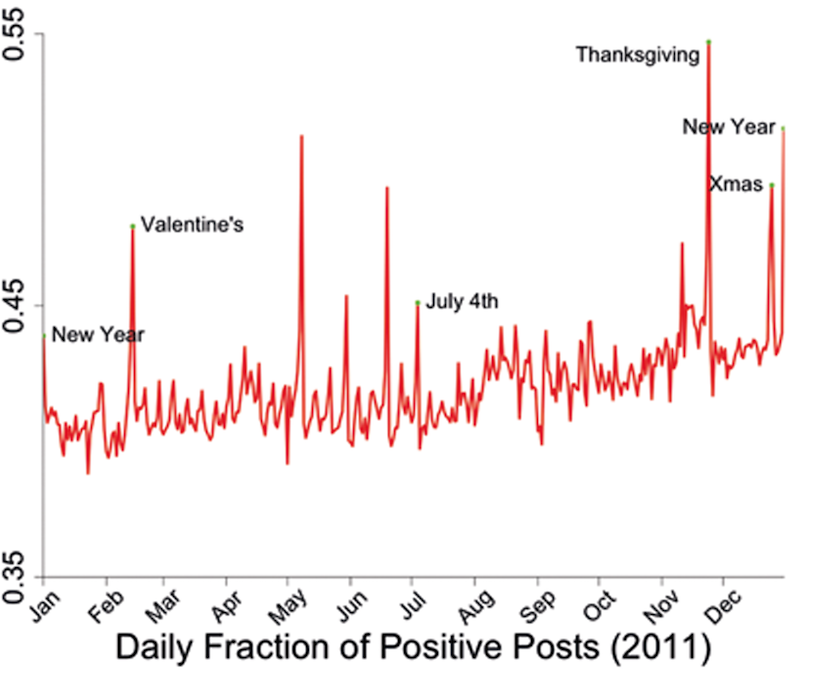
\includegraphics[width=0.5\textwidth]{figures/coviello_detecting_2014_fig1a}
\end{center}

\href{https://doi.org/10.1371/journal.pone.0090315}{Coviello, et al 2014, Fig 1A} 

\end{frame}
%%%%%%%%%%%%%%%%%%%%%%%%%%%
\begin{frame}

Possible solution: Experiment\\  \pause
How could you possibly precisely control the emotional content to which people are exposed and then measure the outcomes?\pause\\
You could work at Facebook.

\begin{center}
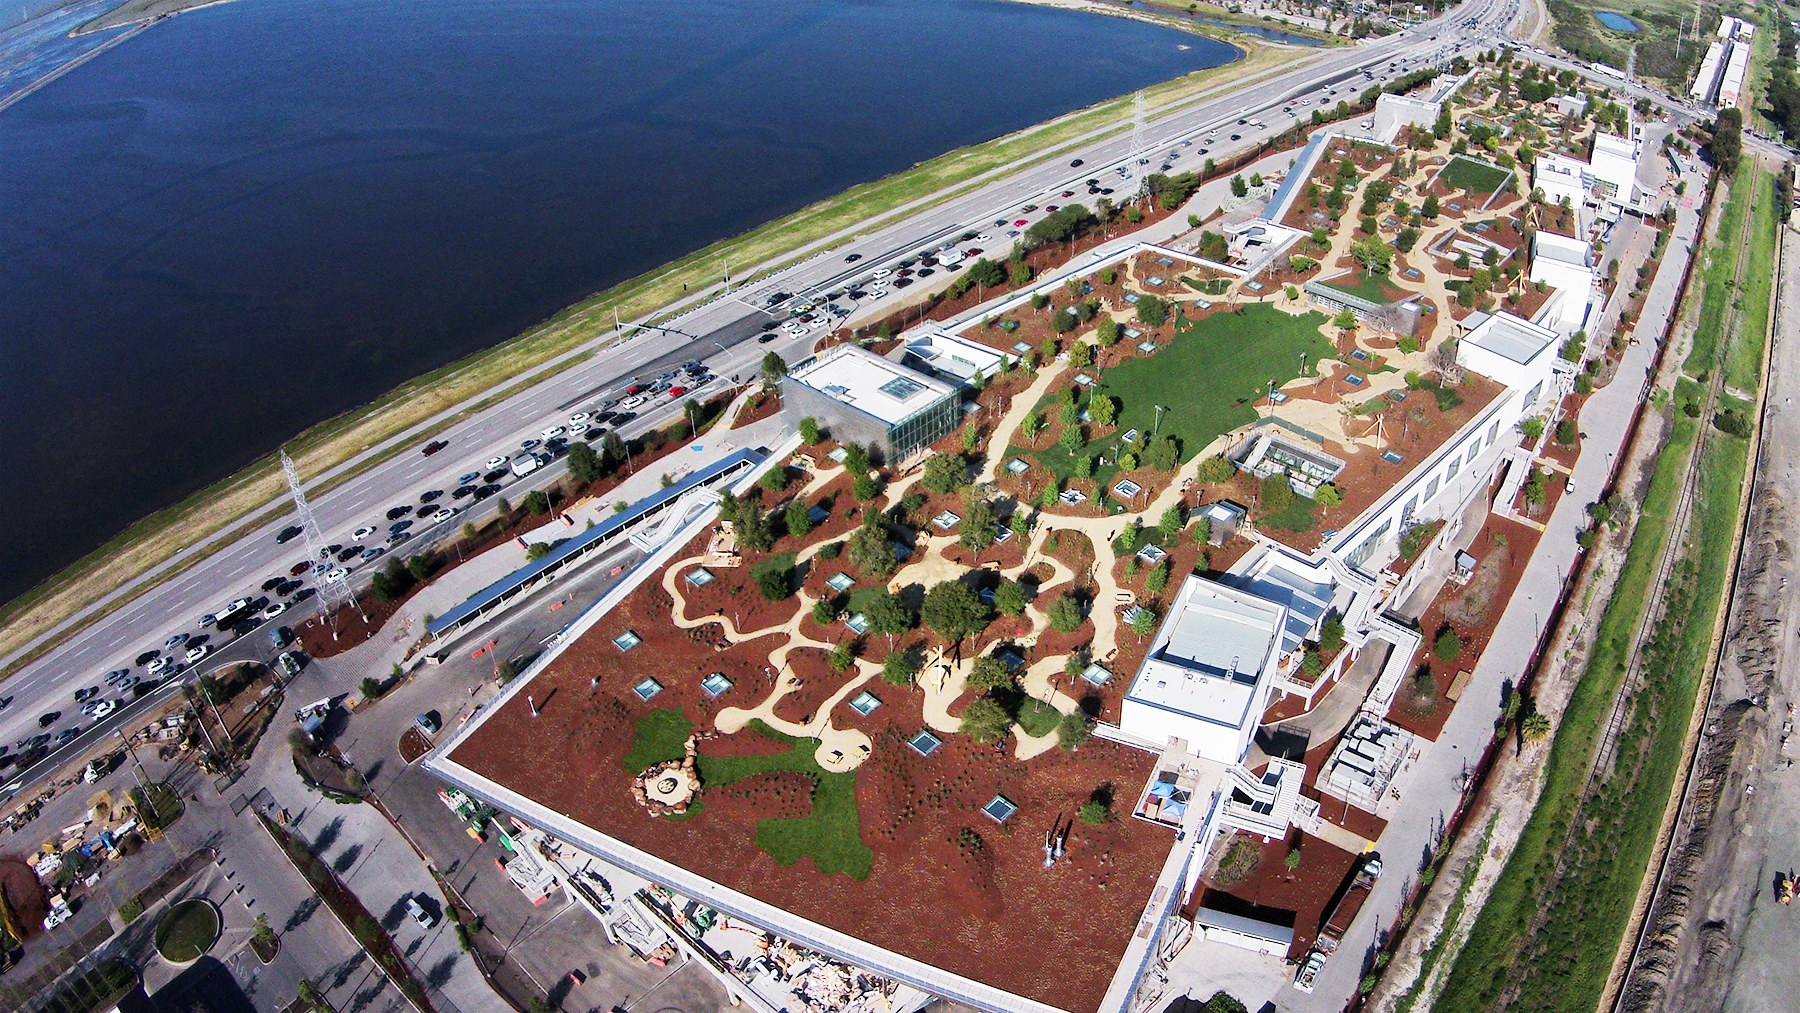
\includegraphics[width=0.5\textwidth]{figures/facebook_hq}
\end{center}

\vfill
\tiny{\url{https://www.wired.com/2015/03/facebook-moves-new-garden-roofed-fantasyland/}}
\end{frame}
%%%%%%%%%%%%%%%%%%%%%%%%%%%
\begin{frame}
\frametitle{Experimental approach}

\begin{center}

\includegraphics[width=\textwidth]{figures/kramer_experimental_2014_title}
\end{center}

\vfill
\url{http://doi.org/10.1073/pnas.1320040111}

\end{frame}
%%%%%%%%%%%%%%%%%%%%%%%%%%%
\begin{frame}

\begin{center}
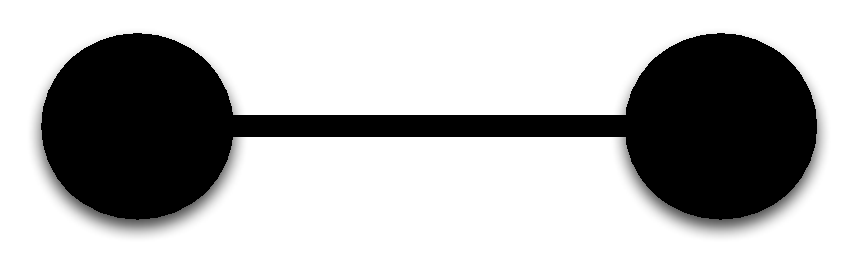
\includegraphics[width=0.8\textwidth]{figures/dyad}
\end{center}

This design works by changing the edge, not by intervene and spillover

\end{frame}
%%%%%%%%%%%%%%%%%%%%
\begin{frame}

Experimental design:
\begin{itemize}
\item 700,000 people
\pause
\item four arms: positive posts reduced vs control, negative posts reduced vs control 
\pause
\item incoming post scored as positive or negative if they had one positive or negative word as defined by Linguistic Inventory and Word Count (LIWC) (e.g., good, sad, etc)
\pause
\item posts randomly blocked from NewsFeed depending on condition (blocking not boosting) 
\pause
\item outcome: percentage of words posted that were positive or negative
\end{itemize}

\vfill
This exact design requires cooperation from Facebook. More generally, many studies of social media's impact require cooperation from social media companies.

\end{frame}
%%%%%%%%%%%%%%%%%%
\begin{frame}

\begin{center}
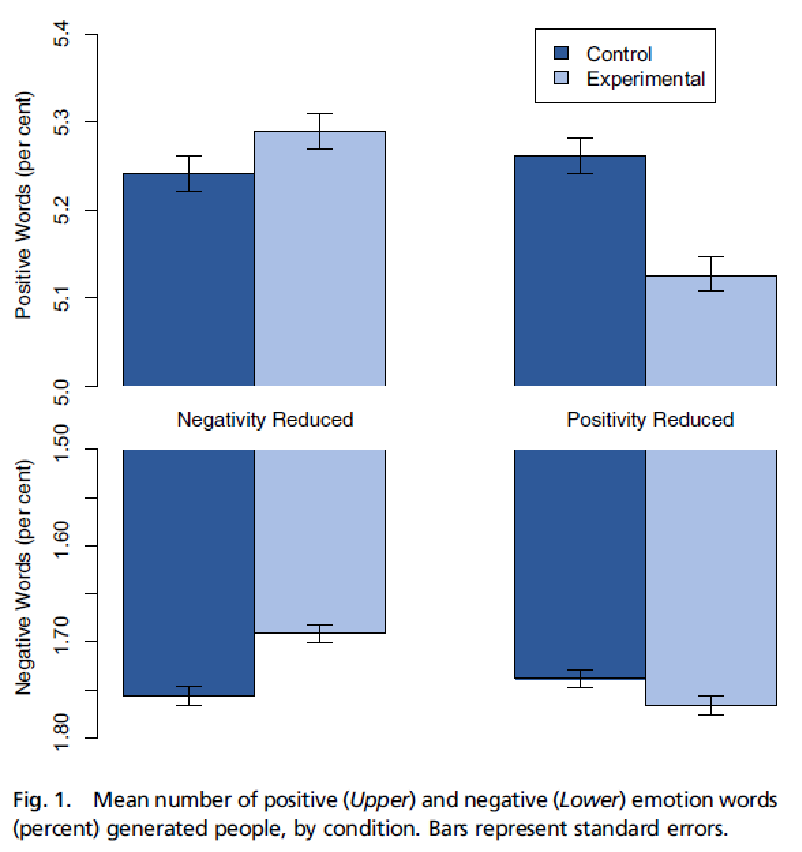
\includegraphics[width=0.5\textwidth]{figures/kramer_experimental_2014_fig1}
\end{center}

\end{frame}
%%%%%%%%%%%%%%%%%%%%%
\begin{frame}

\begin{center}
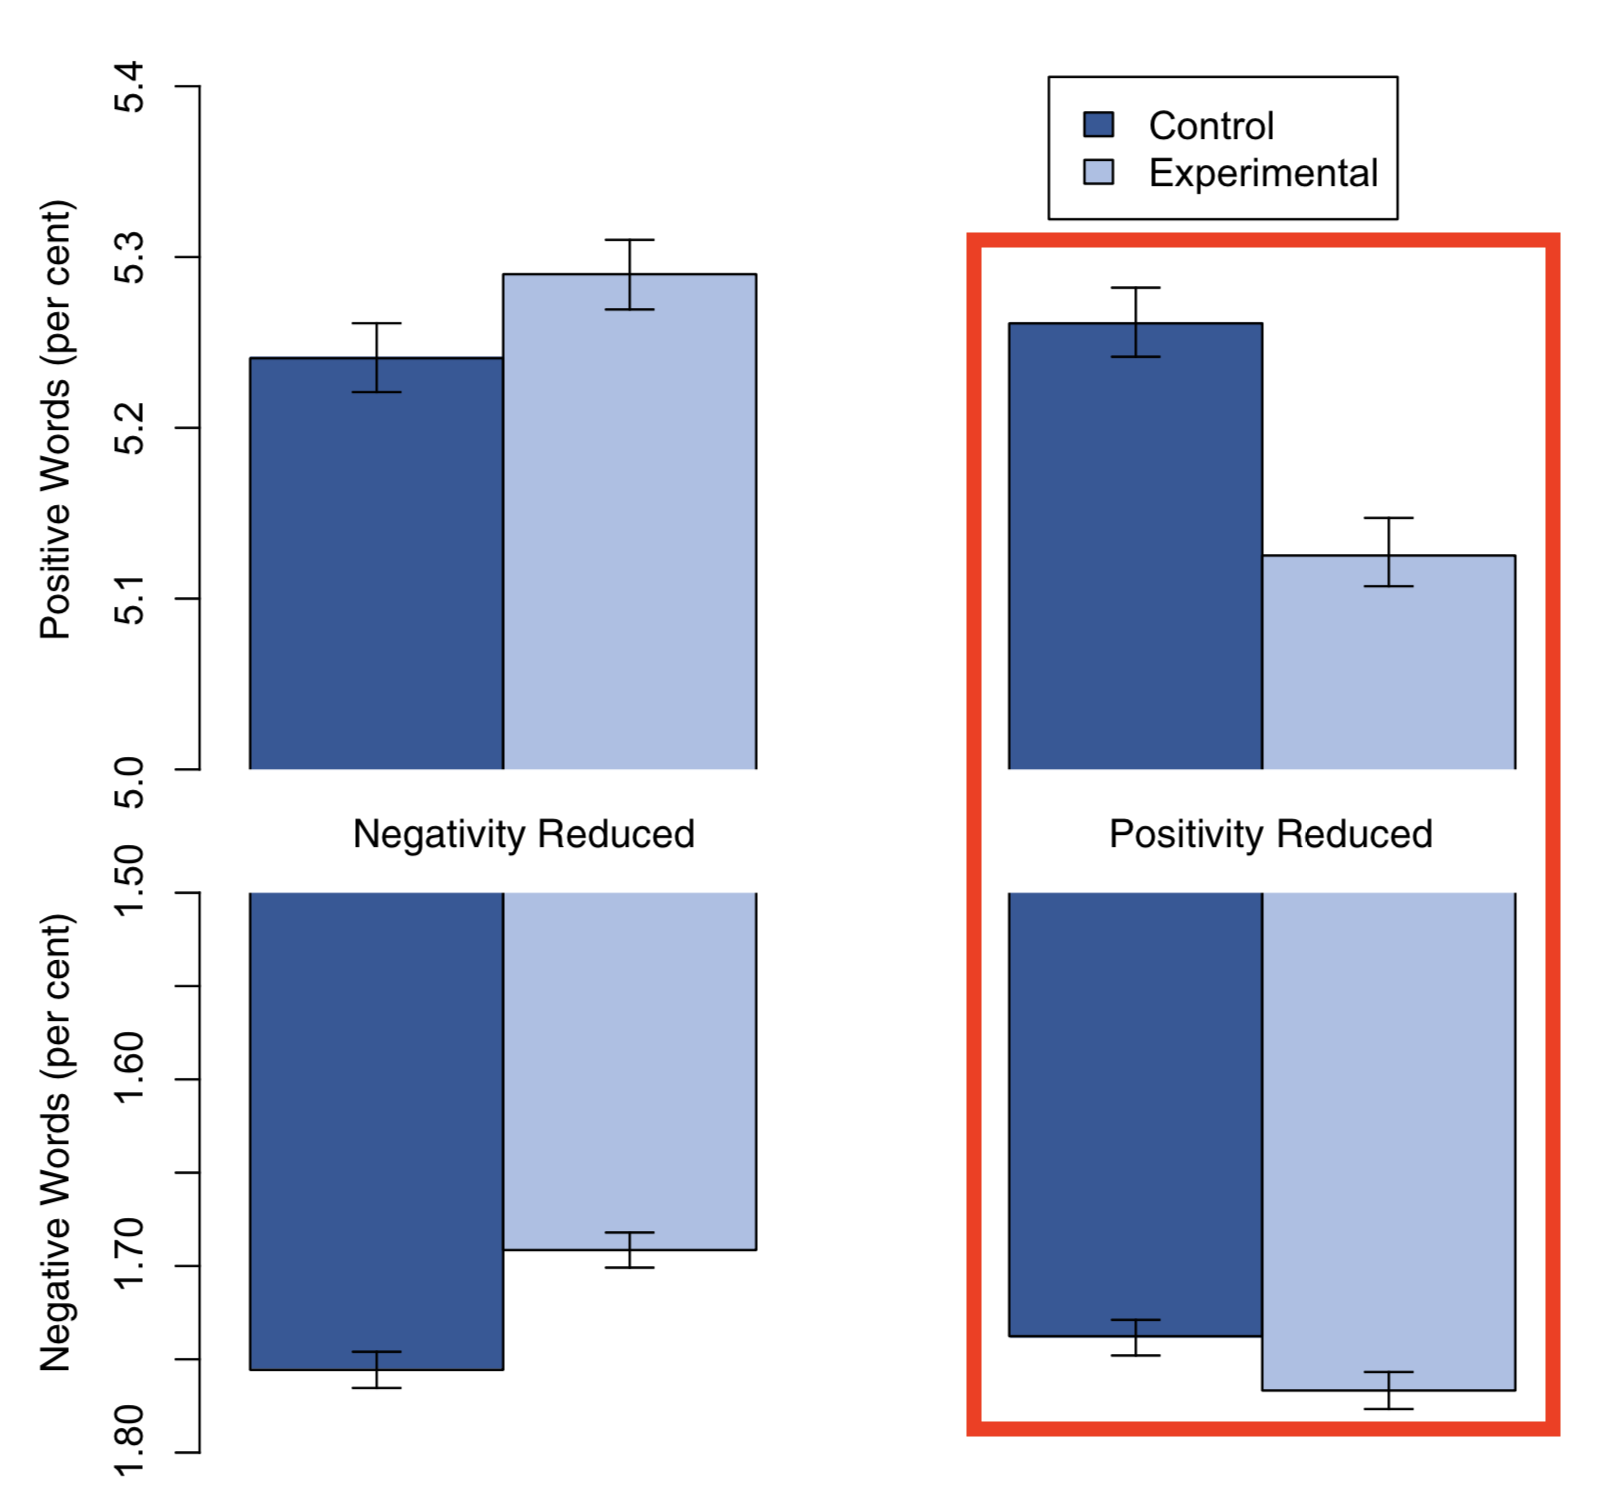
\includegraphics[width=0.2\textwidth]{figures/kramer_experimental_2014_fig1_positivity_reduced}
\end{center}

\begin{itemize}
\item \% positive words in positivity reduced treatment: $\sim$ 5.13\% (5.13 words per 100)
\item \% positive words in positivity reduced control: $\sim$5.27\% (5.27 words per 100)
\item Difference \% positive words: $\sim$-0.14\% (0.14 words per 100, 14 words per 10,000) 
\end{itemize}

\pause

\begin{itemize}
\item \% negative words in positivity reduced treatment: $\sim$1.76\% (1.76 words per 100)
\item \% negative words in positivity reduced control: $\sim$1.74\% (1.74 words per 100)
\item Difference \% negative words: $\sim$0.02\% (0.02 words per 100, 2 words per 10,000) 
\end{itemize}

\note{ 
These are approximate because I just read them off the graph. In the paper they report the results of a more complex analysis
}

\end{frame}
%%%%%%%%%%%%%%%%%%%%%
\begin{frame}

\begin{center}
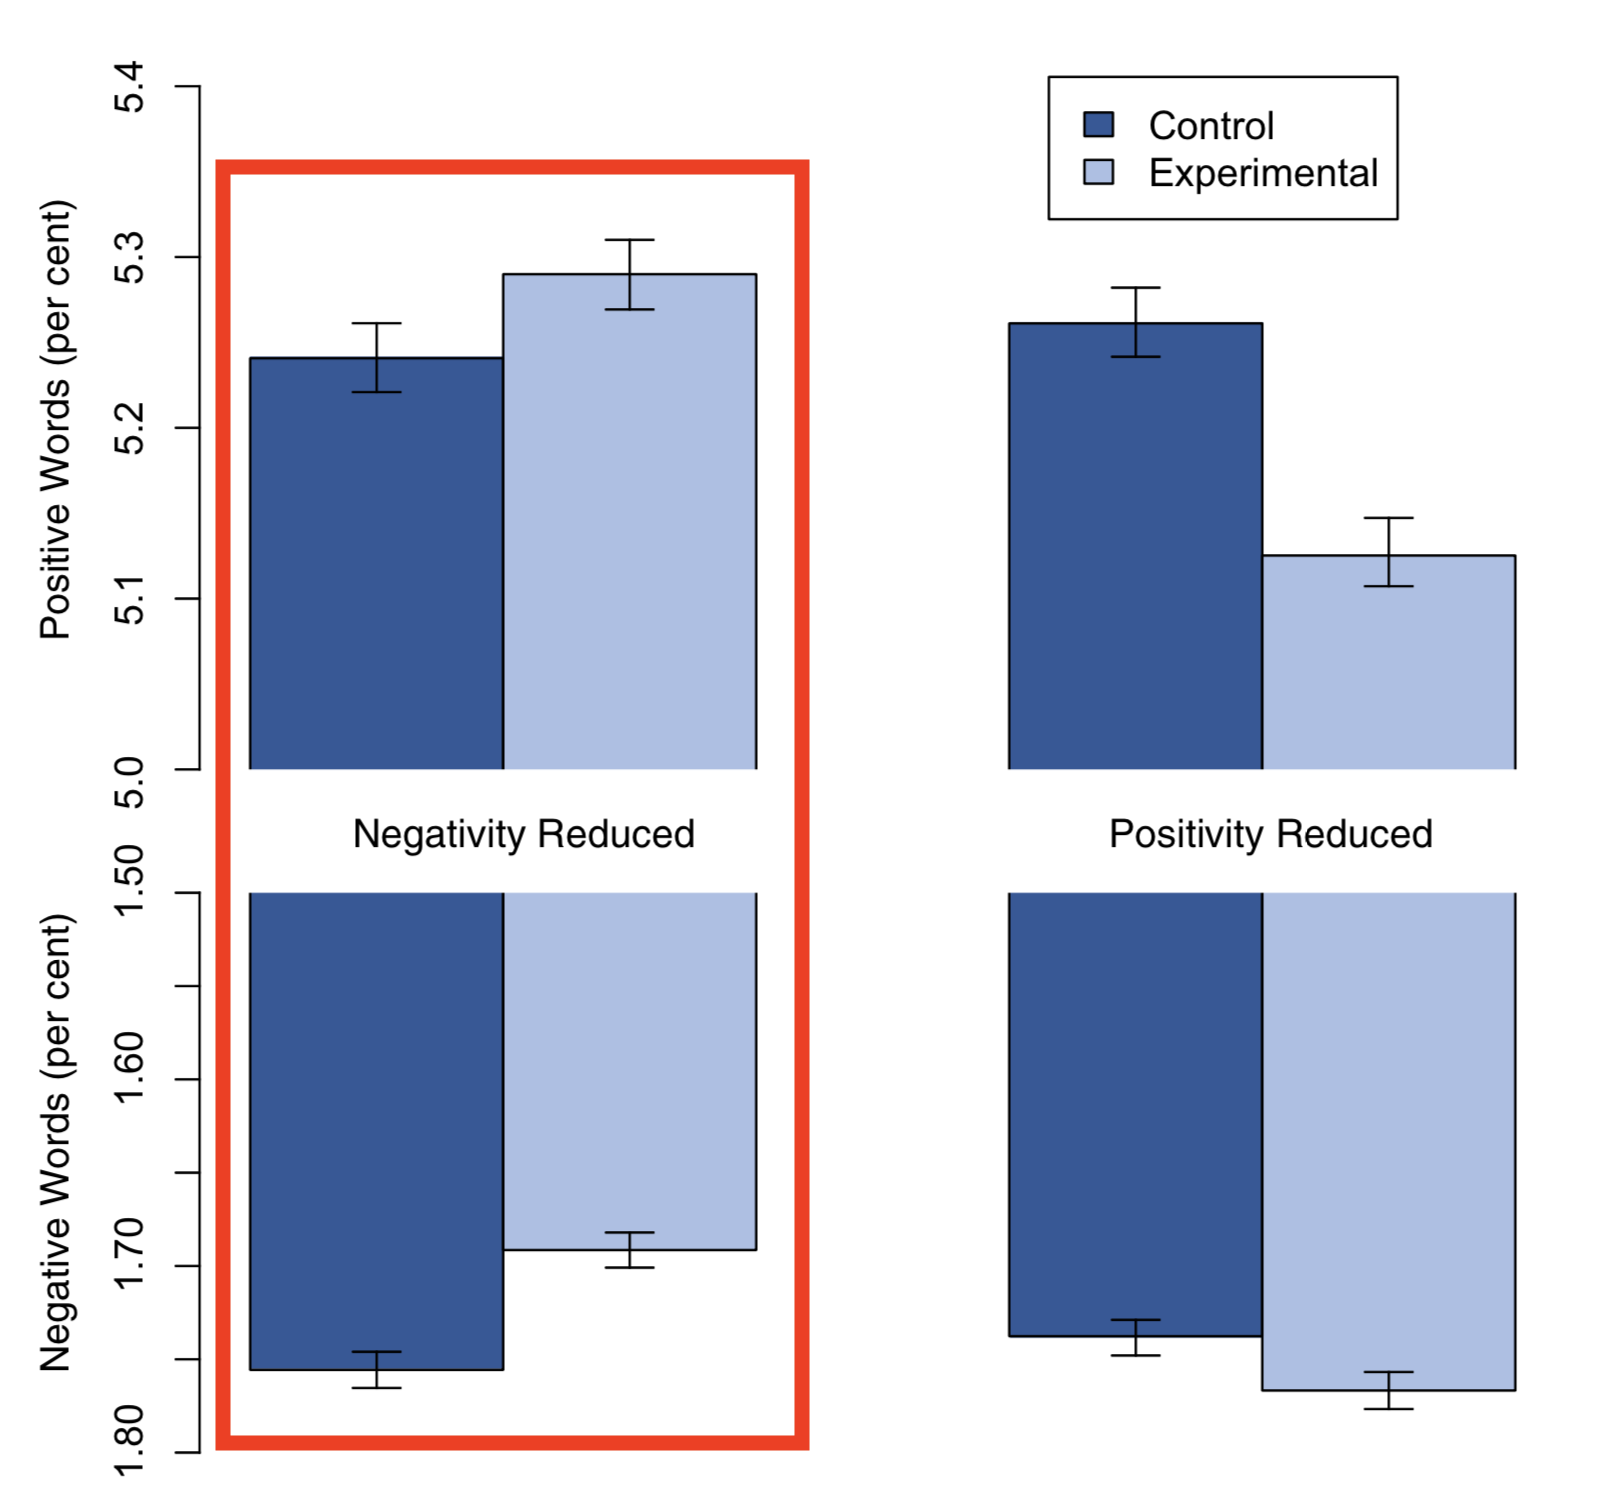
\includegraphics[width=0.2\textwidth]{figures/kramer_experimental_2014_fig1_negativity_reduced}
\end{center}

\begin{itemize}
\item \% positive words in negativity reduced treatment: $\sim$5.29\% (5.29 words per 100)
\item \% of positive words in negativity reduced control: $\sim$5.23\% (5.23 words per 100)
\item Difference \% positive words: $\sim$0.06\% (0.06 words per 100, 6 words per 10,000) 
\end{itemize}

\pause

\begin{itemize}
\item \% negative words in negativity reduced treatment: $\sim$1.69\% (1.69 words per 100)
\item \% negative words in negativity reduced control: $\sim$1.76\% (1.76 words per 100)
\item Difference \% negative words: $\sim$-0.07\% (0.07 words per 100, 7 words per 10,000) 
\end{itemize}

\note{ 
These are approximate because I just read them off the graph. In the paper they report the results of a more complex analysis
}

\end{frame}
%%%%%%%%%%%%%%%%%%%%%
\begin{frame}

How much should you trust these results? Internal and external validity

\end{frame}
%%%%%%%%%%%%%%%%%%%%%
\begin{frame}

Internal validity:
\begin{itemize}
\item Was the randomization delivered correctly?
\item Was the outcome measured correctly on the right people?
\end{itemize}

\pause

\begin{center}
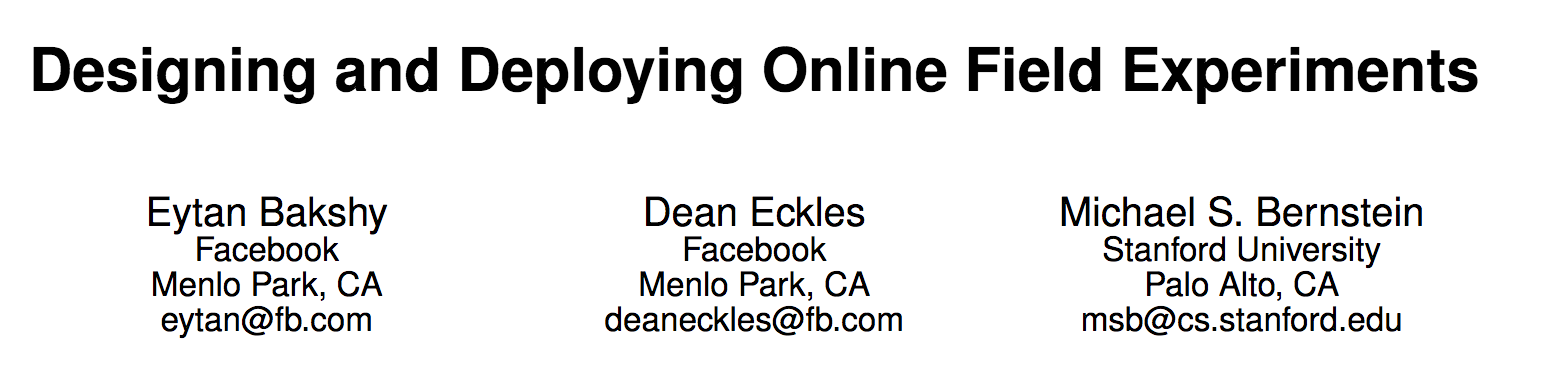
\includegraphics[width=0.8\textwidth]{figures/bakshy_designing_2014_title}
\end{center}

\url{https://arxiv.org/pdf/1409.3174v1.pdf}

\end{frame}
%%%%%%%%%%%%%%%%%%%%%
\begin{frame}
\frametitle{External validity}

External validity:
\begin{itemize}
\item Are Facebook posts a good measure of how we feel?
\pause
\item Is word counts a good way to quantify the emotional content of posts? (``I am so so happy'' vs ``I wish I was happy'')
\end{itemize}
\pause
Probably a bad measure of a bad signal
\end{frame}
%%%%%%%%%%%%%%%%%%%
\begin{frame}

Three other important things about this experiment
\begin{itemize}
\item unintended impact of treatment
\end{itemize}

\end{frame}
%%%%%%%%%%%%%%%%%%%%%%%%%%%%%%%
\begin{frame}

People who had positivity reduced and people who had negativity reduced, posted fewer words.\\

\pause
\vfill
Your treatment can effect your outcome, but also many other outcomes

\end{frame}
%%%%%%%%%%%%%%%%%%%%%
\begin{frame}

\begin{center}
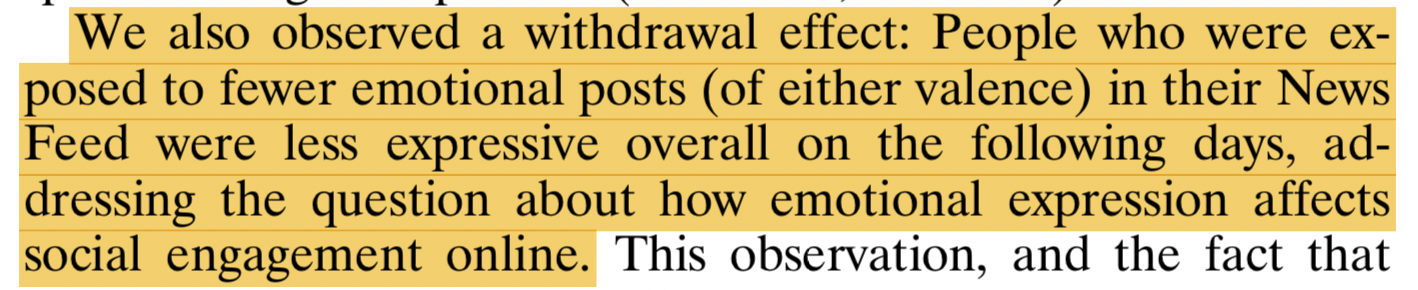
\includegraphics[width=\textwidth]{figures/kramer_experimental_2014_withdraw_effect}
\end{center}
\vfill
Imagine that you work at Facebook and your metric was to increase engagement. \pause Would you adjust the NewsFeed to show more emotional content, either accidentally or intentionally?  

\end{frame}
%%%%%%%%%%%%%%%%%%%%%
\begin{frame}

Three other important things about this experiment
\begin{itemize}
\item unintended impact of treatment
\item ``significance''
\end{itemize}

\end{frame}
%%%%%%%%%%%%%%%%%%%%%%%%%%%%%%%
\begin{frame}

\begin{center}
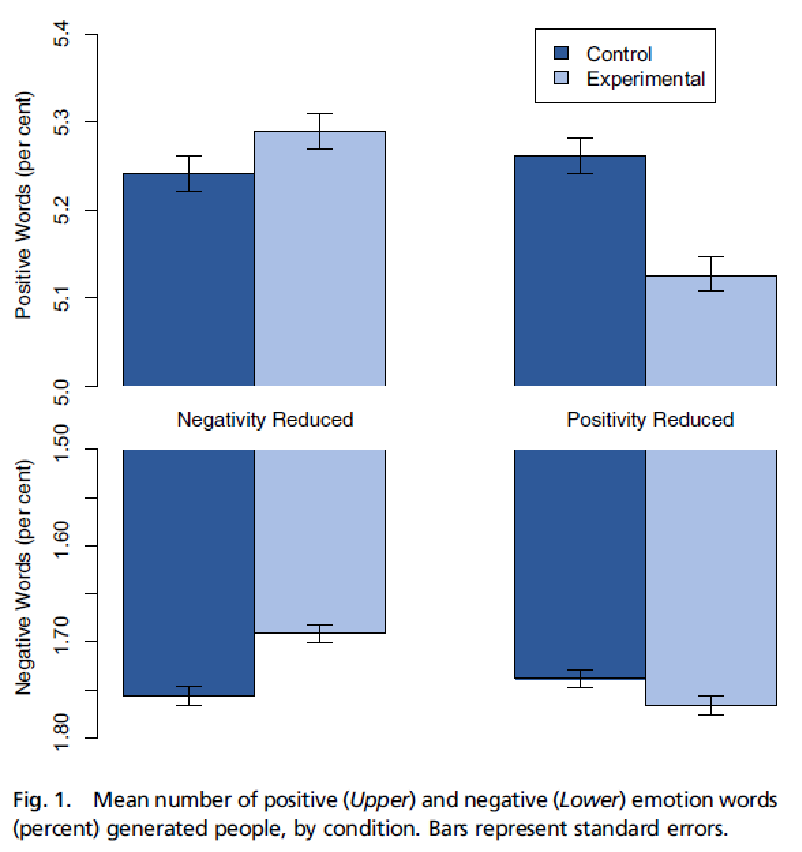
\includegraphics[width=0.4\textwidth]{figures/kramer_experimental_2014_fig1}
\end{center}

\begin{itemize}
\item Are differences that size possible due to chance? (statistical significance)\pause
\item Are differences that big important? (practical importance)
\end{itemize}

\end{frame}
%%%%%%%%%%%%%%%%%%%%%
\begin{frame}

\begin{center}
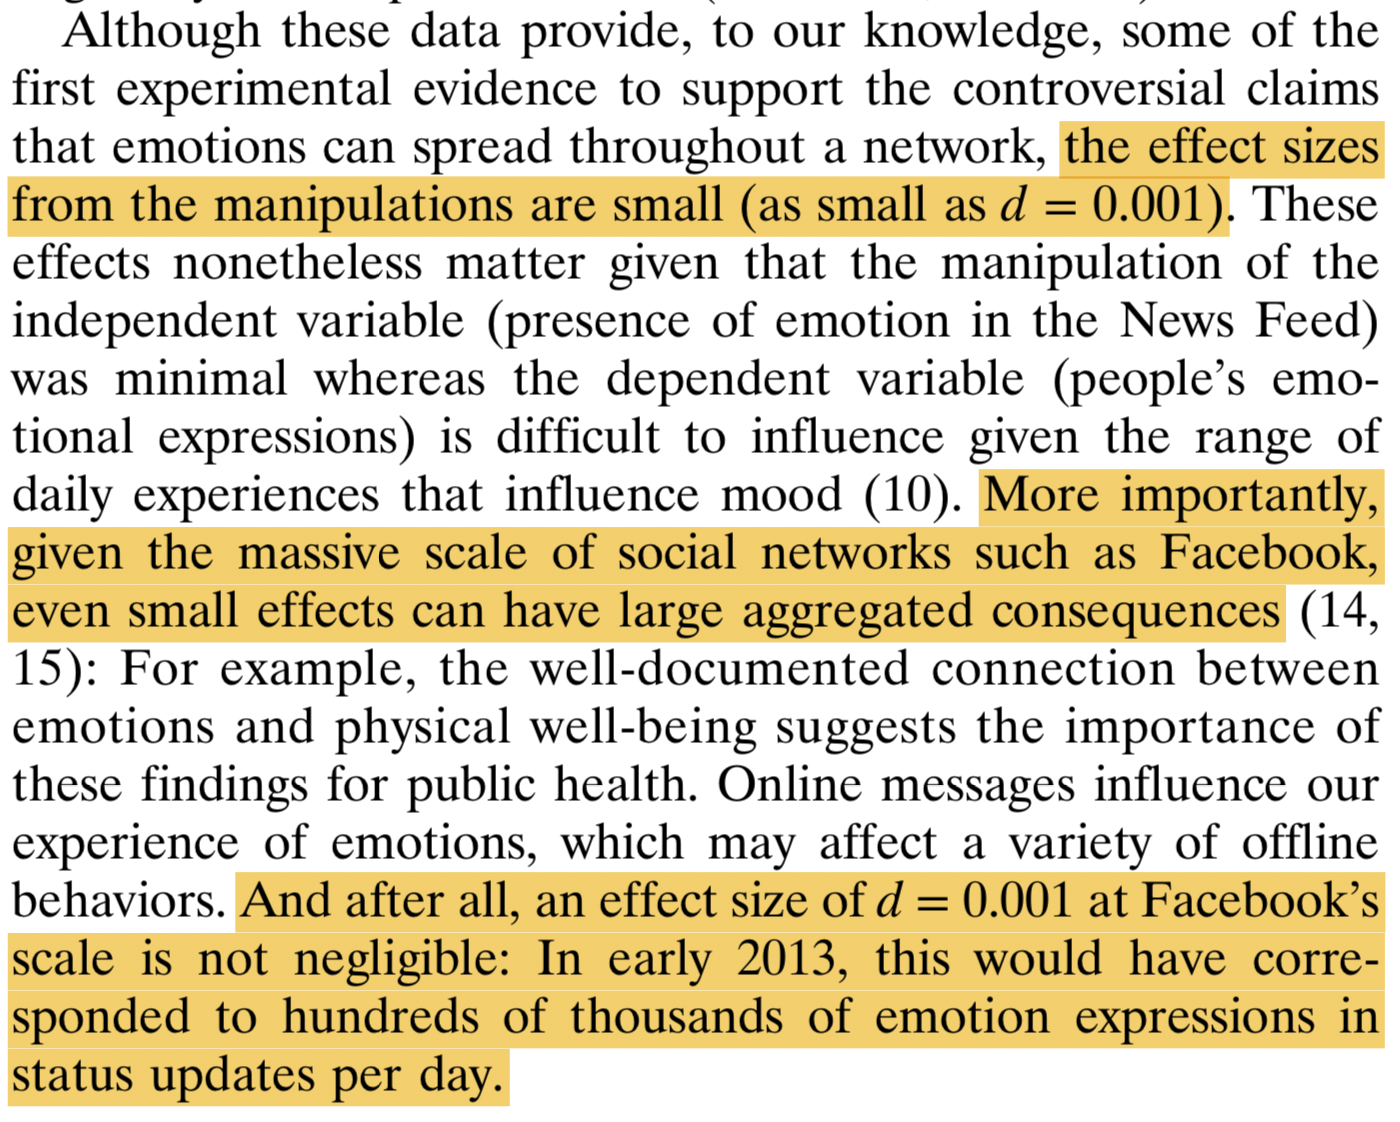
\includegraphics[width=0.65\textwidth]{figures/kramer_experimental_2014_small_effect}
\end{center}

\end{frame}
%%%%%%%%%%%%%%%%%%%%%
\begin{frame}

Three other important things about this experiment
\begin{itemize}
\item unintended impact of treatment
\item ``significance''
\item ethics of running this kind of experiment
\end{itemize}

\end{frame}
%%%%%%%%%%%%%%%%%%%%%%%%%%%%%%%
\begin{frame}

\begin{center}
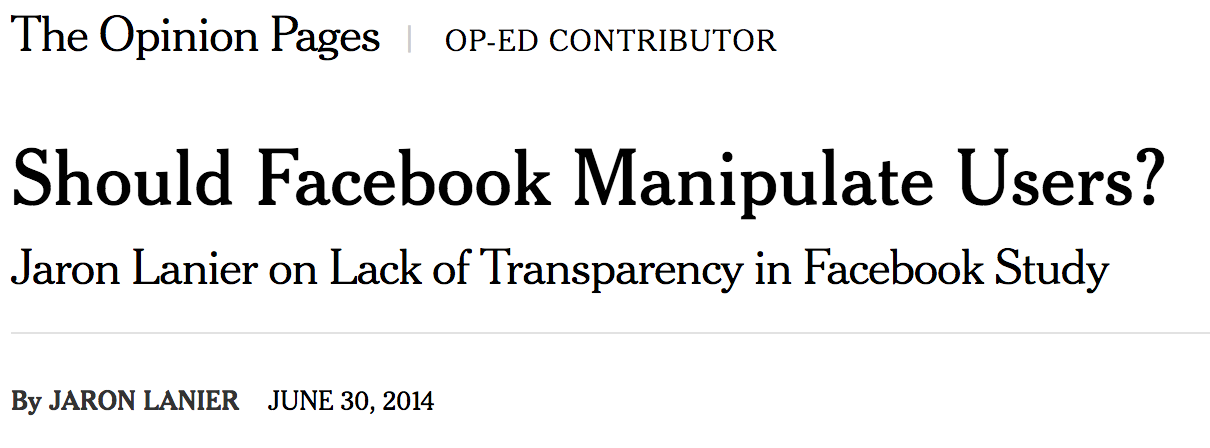
\includegraphics[width=0.8\textwidth]{figures/lanier_should_2014_title}
\end{center}

{\tiny \url{https://www.nytimes.com/2014/07/01/opinion/jaron-lanier-on-lack-of-transparency-in-facebook-study.html}}\\ 

\note{
Some argue that these experiments are unethical
}

\end{frame}
%%%%%%%%%%%%%%%%%%%%%%%%%%%
\begin{frame}

\begin{center}

\includegraphics[width=0.8\textwidth]{figures/watts_stop_2014_title}
\end{center}

{\tiny \url{https://www.theguardian.com/commentisfree/2014/jul/07/facebook-study-science-experiment-research}}\\ 

\note{
Duncan did not write the headline.
Some argue that experiments are permissible or even ethically required
}

\end{frame}
%%%%%%%%%%%%%%%%%%%%%%%%%%%
\begin{frame}

\begin{center}

\includegraphics[height=0.7\textheight]{figures/salganik_bit_2018_cover}
\end{center}

Chapter 6, Ethics: \url{http://www.bitbybitbook.com/en/ethics/}

\end{frame}
%%%%%%%%%%%%%%%%%%%%%%%
%\begin{frame}
%\frametitle{An alternative: Natural experiments}
%
%Possible solution:\\
%Don't randomly assign people to treatments, let nature do it for you.\\\pause
%People post most negative words when it rains.\\
%How do your posts change when it rains in cities where your friends live?
%
%\pause
%
%\begin{center}
%
\includegraphics[width=0.8\textwidth]{figures/coviello_detecting_2014_title}
%\end{center}
%\url{https://doi.org/10.1371/journal.pone.0090315}
%
%\end{frame}
%%%%%%%%%%%%%%%%%%%%%%%%%
\begin{frame}

Experiments are powerful but they are not perfect \pause

\begin{itemize}
\item Powerful: enable us to estimate causal effects (avoid Thanksgiving trap) \pause
\item Not perfect: 
\begin{itemize}
\item potential problems with internal validity
\item potential problems with external validity
\item potential problems with ethics
\end{itemize}
\end{itemize}

\end{frame}
%%%%%%%%%%%%%%%%%%%%%%%%%%%
\begin{frame}

Summary:\\
\begin{itemize}
\item experimental approaches can measure the effect we have on each other
\pause 
\item voting is contagious \& emotional valence of word use is contagious
\pause
\item two designs: 1) intervene and spillover; 2) edge-control
\pause
\item some of these experiments raise ethical questions (e.g., Kramer et al.)
\end{itemize}

\end{frame}
%%%%%%%%%%%%%%%%%%%
\begin{frame}

\LARGE{Going viral}

\end{frame}
%%%%%%%%%%%%%%%%%%%
\begin{frame}

Have you ever said that something was going viral?

\end{frame}
%%%%%%%%%%%%%%%%%%%
\begin{frame}

\begin{itemize}
\item What do viral cascades look like?: Goel, S. et al. (2016). The structural virality of online diffusion. \textit{Management Science} \pause
\item Can they be predicted?: Cheng et al. (2014) Can cascades be predicted? \textit{WWW}
\end{itemize}

\end{frame}
%%%%%%%%%%%%%%%%%%%%

\end{document}
